\documentclass{beamer}
\usepackage{graphicx}
\usepackage[utf8]{inputenc}
\setbeamerfont{institute}{size=\large}
\setbeamerfont{date}{size=\small}

\newcommand\red[1]{\textcolor{red}{#1}}

\usetheme{Madrid}
\usecolortheme{orchid}

\title{Blockchain and Bitcoin}
\subtitle[]{Overview of Blockchain technology and cryptocurrencies, focusing on
the Bitcoin protocol and its scalability and privacy aspects}
\institute[]{Università degli studi di Brescia}
\author{Michele Zanotti}
\date{\today}

\begin{document}
  \begin{frame}
    \titlepage
  \end{frame}

  %%% FIRST SECTION %%%
  \section{Introduction}
  \begin{frame}{Introduction}
    \framesubtitle{Distributed systems}
    \begin{columns}[onlytextwidth]
      \column{.5\textwidth} \begin{block}{Distributed system}
        A \textcolor{red}{distributed system} is a network that consists of autonomous nodes,
        connected using a distribution middleware, which acts in a coordinated way
        (passing messages to each other) in order to achieve a common outcome and
        that can be seen by the user as a single logical platform.
      \end{block}

      \column{.5\textwidth}\begin{figure}[!htb]
        \centering
        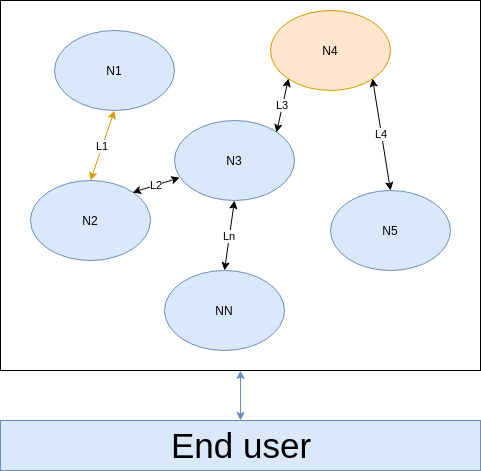
\includegraphics[width=0.7\linewidth]{../img/distributed-system.png}
      \end{figure}
    \end{columns}
  \end{frame}




  \begin{frame}{Introduction}
    \framesubtitle{Distributed systems}
      The desired properties of a distributed system are the following:\vspace{10pt}
      \begin{itemize}
        \item \textbf{Consistency}: all the nodes have the same lates available copy of the data.
        \item \textbf{Availability}: the system is always working and responding to the
        input requests without any failures.
        \item \textbf{Partition tolerance}: if a group of nodes fails the distributed system
        still continues to operate correctly
      \end{itemize}
  \end{frame}




  \begin{frame}{Introduction}
    \framesubtitle{Distributed systems}
    Even if some of the nodes fault or links break, a distributed system should tolerate
    this and should continue to work correctly. There are two types of fault:
    \begin{itemize}
      \item Simple node crash
      \item Exhibition of malicious or inconsistent behavior arbitrarily: \red{Byzantine fault}
    \end{itemize}

    \begin{block}{Byzantine nodes}
      A \textcolor{red}{Byzantine node} is a node that has an arbitrary behavior,
      which can even be malicious.
    \end{block}
  \end{frame}




  \begin{frame}{Introduction}
    \framesubtitle{Distributed systems}
    \begin{block}{Consensus}
      \red{Consensus} is the process of agreement between untrusted nodes on a data
      value.
    \end{block}

    Consensus mechanism requirements:
    \begin{itemize}
      \item \textbf{Agreement}: non-byzantine nodes must agree on the same value
      \item \textbf{Termination}: the consensus process must come to an end (nodes
      have to reach a decision)
      \item \textbf{Validity}: the agreed value must have been proposed by at
      least one honest node
      \item \textbf{Fault tolerance}: the consensus algorithm must work even
      in the presence of one or more Byzantine nodes
    \end{itemize}
  \end{frame}



  \begin{frame}{Introduction}
    \framesubtitle{Distributed systems}
    \begin{block}{The Byzantine generals problem}
     A group of generals are surrounding a city and they have to decide
     whether to attack or retreat. Their only communication way
     is the messenger and they have to agree on a common decision.
     Some of the generals may be traitors trying to prevent the loyal generals
     from reaching an agreement by communicating a misleading message.
     The generals need an algorithm to guarantee that all the loyal generals agree on
     the same plan (attack or retreat) regardless of what traitors generals do.
    \end{block}
  \end{frame}

\end{document}
